\documentclass[]{seti2}

 \usepackage{wrapfig}% embedding figures/tables in text (i.e., Galileo style)
 \usepackage{threeparttable}% tables with footnotes
 \usepackage{dcolumn}% decimal-aligned tabular math columns
  \newcolumntype{d}{D{.}{.}{-1}}
 \usepackage{nomencl}% automatic nomenclature generation via makeindex
 \usepackage{subfigure}% subcaptions for subfigures
 \usepackage{subfigmat}% matrices of similar subfigures, aka small mulitples
 \usepackage{fancyvrb}% extended verbatim environments
  \fvset{fontsize=\footnotesize,xleftmargin=2em}
	\usepackage{lettrine}% dropped capital at beginning of paragraph
	\usepackage[dvipost]{dropping}% alternative dropped capital package
	%\usepackage{hyperref}% embedding hyperlinks [must be loaded after dropping]
	\usepackage[utf8x]{inputenc}
	\usepackage{color}
	\usepackage{graphicx}
	\usepackage{epstopdf}
	\usepackage[brazil]{babel}
	
 \title{TÍTULO DO ARTIGO SUBMETIDO AO IV SETI - SEMINÁRIO EMBRAER DE TECNOLOGIA E INOVAÇÃO}

 \author{
					Elaine Buchalla\\
					{\normalsize\itshape Área Temática: Gestão do Conhecimento }\\
					\and
					Frederico Simões\\
					{\normalsize\itshape Área Temática: Aeronáutica}\\
					\and
					Pedro Ciloni\\
					{\normalsize\itshape Área Temática: Aeronáutica\footnote{\scriptsize{A lista completa de áreas temáticas está apresentada no site: \textcolor[rgb]{0,0,1}{http://eng.embraer.com.br/SETI}}}}\\
				}

\begin{document}

%Título do documento:
\maketitle

%Resumo:
%=============================================================================================
\begin{abstract}
		\underline{\textbf{Resumo}}: O objetivo destas instruções é ser utilizado como um guia para formatação dos artigos a serem submetidos ao V SETI – SEMINÁRIO EMBRAER DE TECNOLOGIA E INOVAÇÃO. O resumo deve descrever os objetivos, a metodologia e as principais conclusões em um único parágrafo, não excedendo 200 palavras. Não deve conter fórmulas e referências bibliográficas
\end{abstract}

\textbf{\textit{Palavras-Chave: Palavra 1, palavra 2 (até 3)}}

%Introdução
%=============================================================================================
\section{INTRODUÇÃO}
  O texto da introdução deverá apresentar o contexto em que o artigo está inserido, seus objetivos e suas justificativas.
	O Artigo\footnote{\scriptsize{Mais informações sobre a estruturação dos artigos estão contidas no site: \textcolor[rgb]{0,0,1}{http://eng.embraer.com.br/SETI/SETI/01.html-website/submissao\_artigos.html}.}} deve ser escrito em no máximo 25 páginas, incluindo Texto, Tabelas e/ou Figuras. 
	A formatação deve seguir tamanho do papel A4, espaçamento entre linhas Simples, formatação do texto Justificado e margens superior, esquerda e direita de 25 mm e inferior 20 mm  (conforme modelo).
	A língua oficial do congresso é o Português, entretanto serão aceitos artigos em Inglês. Porém, as apresentações deverão ser realizadas em Português. 
	Os artigos devem ser rigorosamente formatados de acordo com estas instruções.

%Metodologia
%=============================================================================================
\section{METODOLOGIA}
Indicar sucintamente a metodologia utilizada no desenvolvimento do artigo.

%Resultados
%=============================================================================================
\section{RESULTADOS}
Apresentar os principais resultados obtidos no trabalho, podendo ser utilizados gráficos, tabelas e outras ilustrações necessárias à compreensão do tema.
As equações devem ser apresentadas conforme mostrado pelas Equações \ \ref{e:newton} e \ \ref{e:eq2}.

\begin{equation}
		\label{e:newton}
		F=m\alpha
\end{equation}

\begin{equation}
		\label{e:eq2} % Este label sera usado para referenciar a equação em algum(s) ponto(s) do texto
		B=\mu_{0}.(H+M)	
\end{equation}

As figuras devem ser referenciadas seqüencialmente na parte inferior das mesmas, seguidas do título e centralizadas, como mostrado na Figura \ \ref{figuraAEIOU}. É importante que a figura esteja legível. 

\begin{figure}[htbp!]
		\centering
		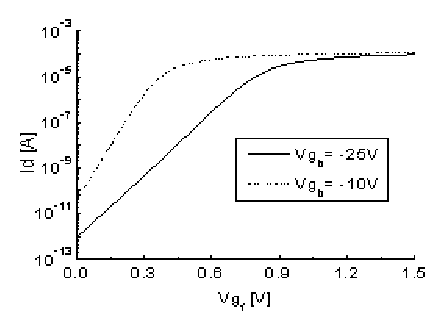
\includegraphics[width=0.5\textwidth]{./figs/Figura1.eps}
		\caption{Título}
		\label{figuraAEIOU}	% Usado para referenciar a figura em algum(s) ponto(s) do texto
\end{figure}

As tabelas devem ser referenciadas seqüencialmente na parte superior das mesmas, seguidas do titulo, como mostrado na Tabela \ \ref{tabelaUOIEA}. O texto da mesma deve ser centralizado.

\begin{table}
		\centering
		\begin{tabular}{|c|c|c|c|}\hline
							& Flaps & Actual & Stage 3 \\ 
							& Setting & Noise Levels & (EPNdB)  \\
							&         & (EPNdB)      &          \\ \hline
			Flyover & 1 & 83.6  & 89.2 \\ \hline
			Lateral & 1 & 92.6  & 95.3 \\ \hline
			Approach & 6 & 92.5  & 99.2 \\ \hline
		\end{tabular}
		\caption{Título}
		\label{tabelaUOIEA}
\end{table}

%Comentários e Conclusões
%=============================================================================================
\section{COMENTÁRIOS E CONCLUSÕES}
Destacar as principais contribuições do autor e indicar, de forma objetiva, as conclusões obtidas.

\vspace{\baselineskip} % Comando para saltar linha (não precisa ter no Artigo final)
\vspace{\baselineskip} % Comando para saltar linha (não precisa ter no Artigo final)

\underline{\textbf{Referências:}}As referências devem ser indicadas ao longo do texto no formato Schutz (1997) ou (SCHUTZ, 1997) e descritas no final do artigo. Devem ser listados apenas os artigos mencionados no texto, em ordem alfabética do sobrenome, pelo primeiro autor. 

A ordem dos itens em cada referência deve obedecer aos exemplos a seguir.
%\underline{Exemplos:}


%Referências bibliográficas
%=============================================================================================
\clearpage %Para que a parte das referências comece em uma nova página
\begin{thebibliography}{50}% maximum number of references (for label width)
			\bibitem{schutz:1997} SCHUTZ, E. \textbf{Reengenharia mental: reeducação de hábitos e programação de metas}. Florianópolis: Insular, 1997. ({\textbf{Exemplo de livro}})
			\bibitem{williams:1950} WILLIAMS, J. W. \textbf{Flow measurement}. In: ROUSE, H. (org.). \textbf{Engineering hydraulics.}. New York: John Wiley \& Sons, 1950. p. 229-309. ({\textbf{Exemplo de capítulo de livro}})
			\bibitem{cup:2003} CIENCIA E OPINIAO. Curitiba: Centro Universitário Positivo. 2003. ({\textbf{Exemplo de periódico}})
			\bibitem{tozzi:2004} TOZZI, M.; OTA, J.  \textbf{Vertedouro em degraus}. Revista da Vinci, Curitiba, v.1, n.1, p. 9-28, 2004. ({\textbf{Exemplo de artigo de periódico}})
			\bibitem{veiga:2001} VEIGA, B. V.  \textbf{Modelagem computacional do processo de eutrofização de aplicação de um modelo de balanço de nutrientes a reservatórios da região metropolitana de Curitiba}. Curitiba, 140 p., 2001. Dissertação (Mestrado) – Universidade Federal do Paraná. ({\textbf{Exemplo de monografia, dissertação e tese}})
			\bibitem{arcdesign:2004} ARC DESIGN. \textbf{Mestres da Arquitetura:} Oscar Niemeyer. São Paulo: Quadrifoglio, n. 35, mar. - abril, 2004. ({\textbf{Exemplo de publicações periódicas consideradas em parte (suplementos, fascículos, números especiais) }})
			\bibitem{moreira:2004} MOREIRA, T. \textbf{Debate sobre software livre chega ao celular}. Valor Econômico, São Paulo, 04 out. 2004. p. B4. ({\textbf{Exemplo de artigo de jornal}})
			\bibitem{yoshida:1996} YOSHIDA, S.; VENDRAMIN, J.C.; OLIVEIRA C. \textbf{Tratamento térmico em matrizes de forjaria em prensas de martelo: como aumentar a vida útil}. In: SEMINÁRIO NACIONAL DE FORJAMENTO, 16., Porto Alegre. Anais... Porto Alegre: UFRGS – Centro de Tecnologia, 1996. p. 29-39 ({\textbf{Exemplo de artigo de jornal}})
			\bibitem{moura:2009} MOURA, G. C. de M. Citação de referências e documentos eletrônicos. Disponível em: \textcolor[rgb]{0,0,1}{http://www.elogica.com.br/users/gmoura/refere.html} Acesso em: 07/01/2009 as 14:00hs. ({\textbf{Exemplo de internet}})
\end{thebibliography}



\end{document}

